\documentclass[11pt]{article}

% ---------------------------------------------------------------- packages
\usepackage[utf8]{inputenc}
\usepackage[T1]{fontenc}
\usepackage[margin=1in]{geometry}
\usepackage{graphicx}
\usepackage{amsmath,amssymb}
\usepackage{booktabs}
\usepackage{microtype}
\usepackage{siunitx}
\usepackage{listings}
\usepackage{xcolor}
\usepackage{tikz}
\usetikzlibrary{arrows.meta,positioning,fit,backgrounds}
\usepackage[hidelinks]{hyperref}
\usepackage{caption}
\usepackage{enumitem}

\graphicspath{{figures/}}

\lstdefinestyle{py}{
  language=Python, basicstyle=\ttfamily\footnotesize,
  keywordstyle=\color{blue!60!black}, commentstyle=\color{green!40!black},
  stringstyle=\color{purple!70!black}, numbers=none, frame=single,
  framesep=4pt, rulecolor=\color{black!25}, showstringspaces=false,
  breaklines=true, columns=fullflexible
}

% ---------------------------------------------------------------- title
\title{\textbf{Globally-Mapped LiDAR Navigation for a Quadruped Robot}\\[2pt]
\large Implementation and Extension of a Classical
Mapping--Localization--Planning Stack}

\author{Sanjit K.\thanks{Undergraduate research intern. Edit author/advisor
fields before submission.}\\
\small Southern Methodist University\\
\small \texttt{akpostme@gmail.com}}

\date{June 22, 2026}

\begin{document}
\maketitle

\begin{abstract}
\noindent
This report documents the implementation and extension of a classical navigation
stack for a quadruped robot operating on uneven terrain, following the
LiDAR mapping $\rightarrow$ localization $\rightarrow$ global planning
$\rightarrow$ local obstacle avoidance architecture of a recent IEEE study
\cite{refpaper}. We build the stack from first principles in Python
(\texttt{numpy}/\texttt{matplotlib} only \cite{harris2020,hunter2007}): a 2.5D
elevation-grid discretization of raw point clouds; a per-cell Kalman-filtered
probabilistic terrain map \cite{kalman1960,fankhauser2018}; a Dijkstra/A$^\star$
global planner \cite{dijkstra1959,hart1968} with elastic-band (Timed-Elastic-Band)
smoothing \cite{rosmann2017}; and an artificial-potential-field (APF) local
planner in the Khatib formulation \cite{khatib1986}. We validate on synthetic
terrain, on real automotive LiDAR from the KITTI dataset \cite{geiger2013}, and on
an indoor RGB-D reconstruction \cite{zhou2018}, and we provide a ROS\,2 / Nav2
integration path \cite{macenski2020,macenski2022}. Beyond reproduction, we add a
moving-goal APF mode aimed at the autonomous \emph{person-following} task
\cite{islam2019}. Experiments expose three practical lessons: (i) traversability
thresholds are sensor-specific, with clean LiDAR working at default settings while
noisy single-view RGB-D requires looser tolerances and stronger smoothing; (ii)
naive multi-scan fusion without scan registration (ICP \cite{besl1992}) inflates
obstacles through ghosting, demonstrating empirically why the reference method
requires a localization stage; and (iii) APF alone is trapped by local minima at
large obstacles, confirming the necessity of the two-level (global + local)
design.
\end{abstract}

% ================================================================
\section{Introduction}
\label{sec:intro}

Legged robots are increasingly deployed on terrain that wheeled platforms cannot
negotiate---construction sites, disaster zones, and natural ground with steps,
slopes, and gaps. Autonomous navigation for such robots requires a terrain
representation that preserves the geometric features relevant to footing, a means
of localizing within that representation, and planners that produce both a
long-range route and reactive avoidance of nearby hazards.

The reference study \cite{refpaper} proposes an integrated stack for a quadruped
that combines established components: a LiDAR-built terrain elevation map refined
by Kalman filtering; SLAM-based localization fusing GPS, IMU, odometry, and LiDAR
with Iterative Closest Point (ICP) scan matching \cite{besl1992}; a Dijkstra
global planner \cite{dijkstra1959} on a grid map smoothed by a Timed-Elastic-Band
(TEB) optimizer \cite{rosmann2017}; and an artificial-potential-field (APF) local
obstacle avoider \cite{khatib1986}. The contribution of \cite{refpaper} is the
\emph{integration} rather than any single new algorithm.

This report reproduces the core of that stack and extends it toward the
research direction of interest---autonomous \emph{person-following}
\cite{islam2019}---where the navigation target is a moving person rather than a
fixed goal. Our contributions are:
\begin{enumerate}[leftmargin=1.4em,itemsep=1pt]
  \item A self-contained 2.5D elevation-grid discretization of raw point clouds
        with robust per-cell statistics and a traversability cost model
        (Sec.~\ref{sec:disc}).
  \item A per-cell Kalman probabilistic terrain map that fuses multiple scans and
        gates untrustworthy cells by variance (Sec.~\ref{sec:kalman}).
  \item Dijkstra/A$^\star$ global planning, elastic-band smoothing, and a Khatib
        APF local planner with a moving-goal (person-following) mode
        (Secs.~\ref{sec:global}--\ref{sec:apf}).
  \item A ROS\,2/Nav2 deployment path that publishes the map as a costmap layer
        (Sec.~\ref{sec:nav2}).
  \item An empirical study on synthetic, automotive-LiDAR, and indoor-RGB-D data
        that surfaces concrete lessons about sensor-specific tuning, scan
        registration, and global/local planner roles (Sec.~\ref{sec:results}).
\end{enumerate}

% ================================================================
\section{Background and Related Work}
\label{sec:related}

\paragraph{Terrain representations.} Occupancy grids \cite{elfes1989} discretize
the environment into free/occupied cells but collapse the vertical dimension. For
legged robots the \emph{2.5D elevation grid}---one height value (and optionally a
variance) per planar cell---retains steps, curbs, and slopes while remaining far
cheaper than full 3D volumetric maps such as OctoMap \cite{hornung2013}.
Robot-centric, uncertainty-aware elevation mapping was formalized by Fankhauser
\emph{et al.} \cite{fankhauser2014,fankhauser2018}, who maintain a Gaussian height
estimate per cell updated by a Kalman filter \cite{kalman1960,thrun2005}.

\paragraph{Planning.} Dijkstra's algorithm \cite{dijkstra1959} computes
shortest-cost paths by uniform-cost expansion; A$^\star$ \cite{hart1968} adds an
admissible heuristic for efficiency. Grid paths are jagged, so trajectory
optimizers such as TEB \cite{rosmann2012,rosmann2017} refine them under geometric
and (for full TEB) kinodynamic constraints. For reactive avoidance, the artificial
potential field \cite{khatib1986} treats the goal as an attractor and obstacles as
repellers; its well-known weakness is entrapment in local minima.

\paragraph{Datasets and tooling.} We evaluate on the KITTI autonomous-driving
benchmark \cite{geiger2012,geiger2013} (Velodyne HDL-64 scans) and on an indoor
RGB-D fragment from Open3D \cite{zhou2018}. Deployment targets ROS\,2 and the Nav2
navigation framework \cite{quigley2009,macenski2020,macenski2022}.

% ================================================================
\section{System Overview}
\label{sec:overview}

Figure~\ref{fig:arch} shows the pipeline. Raw point clouds, assumed expressed in a
stable world frame by the localization stage, are fused into a probabilistic 2.5D
elevation map. The map yields a traversability cost grid consumed by the global
planner; the resulting route is smoothed and tracked by the APF local planner,
which also supports a moving goal for person-following. The localization block
(SLAM/ICP) is treated as an assumed input in this work (Sec.~\ref{sec:limits}).

\begin{figure}[t]
\centering
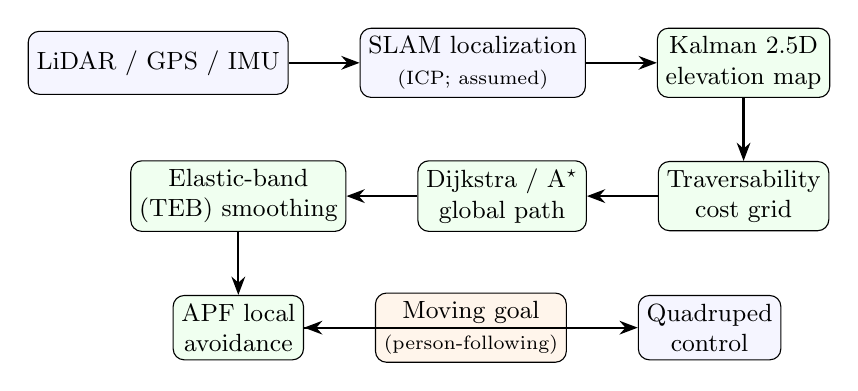
\begin{tikzpicture}[
  node distance=6mm and 9mm,
  box/.style={draw, rounded corners, align=center, minimum height=8mm,
    inner sep=3pt, font=\small, fill=blue!4},
  impl/.style={box, fill=green!6},
  ext/.style={box, fill=orange!8},
  >={Stealth[]}, every edge/.style={draw, ->, thick}]
  \node[box] (sensor) {LiDAR / GPS / IMU};
  \node[box, right=of sensor] (loc) {SLAM localization\\\scriptsize(ICP; assumed)};
  \node[impl, right=of loc] (map) {Kalman 2.5D\\elevation map};
  \node[impl, below=8mm of map] (cost) {Traversability\\cost grid};
  \node[impl, left=of cost] (global) {Dijkstra / A$^\star$\\global path};
  \node[impl, left=of global] (teb) {Elastic-band\\(TEB) smoothing};
  \node[impl, below=8mm of teb] (apf) {APF local\\avoidance};
  \node[ext, right=of apf] (person) {Moving goal\\\scriptsize(person-following)};
  \node[box, right=of person] (ctrl) {Quadruped\\control};
  \draw (sensor) edge (loc);
  \draw (loc) edge (map);
  \draw (map) edge (cost);
  \draw (cost) edge (global);
  \draw (global) edge (teb);
  \draw (teb) edge (apf);
  \draw (person) edge (apf);
  \draw (apf) edge (ctrl);
\end{tikzpicture}
\caption{System architecture. Green blocks are implemented in this work; the
orange block is the person-following extension; the localization block (white) is
assumed. The structure follows the reference stack \cite{refpaper}.}
\label{fig:arch}
\end{figure}

% ================================================================
\section{2.5D Elevation Discretization}
\label{sec:disc}

A point cloud $\{(x_k,y_k,z_k)\}_{k=1}^{N}$ is binned into a grid of resolution
$r$. For a cell with the set of contained returns $\mathcal{Z}$, we accumulate
count, sum, and sum-of-squares in a single vectorized pass and derive a
\emph{robust} per-cell elevation and roughness:
\begin{equation}
\hat h = \frac{1}{|\mathcal{Z}|}\sum_{z\in\mathcal{Z}} z, \qquad
\sigma_{\text{cell}} = \sqrt{\;\mathbb{E}[z^2]-\mathbb{E}[z]^2\;}.
\label{eq:rough}
\end{equation}
Using the standard deviation~\eqref{eq:rough} rather than the raw range
$\max z-\min z$ makes roughness insensitive to a single stray return and to point
density. Slope is the magnitude of the elevation gradient, computed in a
NaN-aware manner so cells adjacent to map holes are not corrupted:
\begin{equation}
s = \lVert \nabla \hat h \rVert,\qquad
\Delta = \max_{j\in\mathcal{N}_4} \lvert \hat h - \hat h_j\rvert,
\label{eq:slopestep}
\end{equation}
where $\Delta$ is the maximum height difference to the four-connected neighbours
(a discrete step detector, following the grid height-difference test of
\cite{refpaper}). A cell is classified \textsc{lethal} if it exceeds the robot's
mobility limits (Table~\ref{tab:params}):
\begin{equation}
\textsc{lethal} \iff \Delta > \Delta_{\max} \;\lor\; s > \tan\theta_{\max}
\;\lor\; \sigma_{\text{cell}} > \sigma_{\max}.
\label{eq:lethal}
\end{equation}
Isolated lethal cells (sensor speckle) are removed by dropping connected
components smaller than three cells---this, unlike morphological opening, does not
thin genuine thin walls. Surviving obstacles are dilated by the footprint radius
for clearance. The continuous cost combines smooth penalties with a lethal
sentinel:
\begin{equation}
c = 1 + w_s\frac{s}{\tan\theta_{\max}} + w_r\frac{\sigma_{\text{cell}}}{\sigma_{\max}},
\qquad c \leftarrow \infty \text{ if \textsc{lethal}.}
\label{eq:cost}
\end{equation}

\begin{table}[t]
\centering
\caption{Default quadruped mobility parameters (Go2/Spot class).}
\label{tab:params}
\begin{tabular}{llr}
\toprule
Symbol & Meaning & Default \\
\midrule
$\rho_{\text{body}}$   & footprint radius (inflation) & \SI{0.30}{m} \\
$\Delta_{\max}$        & maximum climbable step       & \SI{0.18}{m} \\
$\theta_{\max}$        & maximum traversable slope    & \ang{30} \\
$\sigma_{\max}$        & maximum within-cell height std & \SI{0.05}{m} \\
$r$                    & grid resolution               & \SI{0.10}{m} \\
\bottomrule
\end{tabular}
\end{table}

% ================================================================
\section{Probabilistic Terrain Mapping with a Kalman Filter}
\label{sec:kalman}

Each cell maintains a height estimate $\hat h$ and variance $P$. A LiDAR return at
range $\varrho$ from the sensor is assigned a measurement variance that grows with
range,
\begin{equation}
R = \sigma_0^2 + \alpha\,\varrho^2,
\label{eq:measvar}
\end{equation}
reflecting the degradation of LiDAR depth accuracy with distance. Multiple returns
landing in one cell during a single scan are combined in information form before
the update,
\begin{equation}
\bar z = \frac{\sum_k z_k/R_k}{\sum_k 1/R_k},\qquad
\bar R = \frac{1}{\sum_k 1/R_k}.
\label{eq:combine}
\end{equation}
The cell is then updated by the scalar Kalman filter
\cite{kalman1960,thrun2005,fankhauser2018}:
\begin{align}
\text{(init, } P=\infty\text{):}\quad & \hat h \leftarrow \bar z,\quad P \leftarrow \bar R, \label{eq:kinit}\\
\text{(update):}\quad & K = \frac{P}{P+\bar R},\quad
   \hat h \leftarrow \hat h + K(\bar z - \hat h),\quad
   P \leftarrow (1-K)P. \label{eq:kupdate}
\end{align}
A prediction step $P \leftarrow P + q$ injects process noise so the map remains
adaptive to change. Listing~\ref{lst:kalman} shows the implementation core. A
subtle but important detail: the prior-finite mask must be captured \emph{before}
mutating the height array, otherwise a cell's first observation is both
initialized and fused against itself, incorrectly halving its variance.

\begin{lstlisting}[style=py, caption={Per-cell Kalman fusion (information-form combine then scalar update).}, label={lst:kalman}]
had  = np.isfinite(self.height)        # snapshot BEFORE mutating
fresh = observed & ~had                # first observation -> initialize
self.height[fresh]   = z_meas[fresh]
self.variance[fresh] = R_meas[fresh]
upd = observed & had                   # fuse with existing estimate
P, R = self.variance[upd], R_meas[upd]
K = P / (P + R)
self.height[upd]   += K * (z_meas[upd] - self.height[upd])
self.variance[upd]  = (1.0 - K) * P
\end{lstlisting}

The fused map is converted to a cost grid via
Eqs.~\eqref{eq:slopestep}--\eqref{eq:cost}, with the addition of a
\emph{variance gate}: cells whose variance remains above a threshold are labelled
\textsc{unknown} rather than trusted, so the planner does not commit to poorly
observed ground.

% ================================================================
\section{Global Path Planning and Smoothing}
\label{sec:global}

Following \cite{refpaper} we plan globally with Dijkstra's algorithm
\cite{dijkstra1959} over the cost grid; we also provide A$^\star$ \cite{hart1968}
with the octile heuristic for efficiency. Both are 8-connected, and the cost of
traversing from cell $u$ to neighbour $v$ is the mean cell cost scaled by the step
distance:
\begin{equation}
g(u\!\to\!v) = d(u,v)\cdot\tfrac{1}{2}\big(c_u + c_v\big),\quad
d\in\{1,\sqrt2\}.
\label{eq:edge}
\end{equation}
Dijkstra is exactly A$^\star$ with a zero heuristic; a unit test confirms the two
return paths of identical cost. The raw grid path is then geometrically smoothed
by an elastic band---the geometric core of TEB \cite{rosmann2017}. Each interior
waypoint $p_i$ is pulled toward the midpoint of its neighbours (contraction) and
pushed away from obstacles within an influence distance via the gradient of a
chamfer distance field $D$:
\begin{equation}
p_i \leftarrow p_i + \underbrace{w_c\big(p_{i-1}+p_{i+1}-2p_i\big)}_{\text{smoothness}}
 + \underbrace{w_o\,\max\!\Big(0,\tfrac{d_0-D(p_i)}{d_0}\Big)\widehat{\nabla D}}_{\text{clearance}}.
\label{eq:eband}
\end{equation}
Endpoints are fixed and any waypoint that would enter an obstacle cell is rejected.
We note explicitly that this is the geometric stand-in for TEB; the full
time-optimal, kinodynamic TEB of \cite{rosmann2017} is left to future work.

% ================================================================
\section{Local Obstacle Avoidance (APF) and Person-Following}
\label{sec:apf}

The local planner uses the Khatib potential field \cite{khatib1986}. With robot
position $q$ and goal $q_g$, the attractive force (with a conic far-field cap to
avoid huge forces at long range) and the repulsive force from the nearest obstacle
at distance $\varrho$ within influence radius $\varrho_0$ are
\begin{align}
F_{\text{att}} &= k_a\,(q_g - q), \label{eq:fatt}\\
F_{\text{rep}} &=
\begin{cases}
k_r\Big(\dfrac{1}{\varrho}-\dfrac{1}{\varrho_0}\Big)\dfrac{1}{\varrho^2}\,\widehat{\nabla\varrho}, & \varrho \le \varrho_0,\\[6pt]
0, & \varrho > \varrho_0,
\end{cases}
\label{eq:frep}
\end{align}
and the robot integrates $q \leftarrow q + \mathrm{clip}(F_{\text{att}}+F_{\text{rep}},\,v_{\max})\,\Delta t$.
Obstacle distance $\varrho$ and its gradient come from a chamfer distance field, so
each force query is $O(1)$.

\paragraph{Two-level operation.} Pure APF toward a distant goal is trapped by
local minima at large obstacles (Sec.~\ref{sec:results}). The faithful
architecture therefore tracks the global path with a moving \emph{carrot} sub-goal
a fixed look-ahead ahead of the robot, so the attractive force never points
through a wall while repulsion still trims hazards.

\paragraph{Person-following.} For the target application the goal is a moving
person, modelled as $q_g(t)$, a callable of time \cite{islam2019}. The same APF
loop tracks $q_g(t)$ directly while repulsion avoids terrain hazards; the global
Dijkstra planner becomes secondary because the destination is no longer fixed.

% ================================================================
\section{ROS\,2 / Nav2 Integration}
\label{sec:nav2}

For deployment, a ROS\,2 (Humble) node subscribes to a \texttt{PointCloud2},
discretizes it, and republishes a \texttt{nav\_msgs/OccupancyGrid} that Nav2
\cite{macenski2020,macenski2022} consumes through a \texttt{StaticLayer}. To avoid
double inflation, the node publishes the un-inflated traversability grid and lets
Nav2's \texttt{InflationLayer} apply footprint clearance; the soft slope/roughness
costs are preserved by setting \texttt{trinary\_costmap:\,false}. This keeps the
numpy core unchanged and reuses Nav2's mature planners and controllers.

% ================================================================
\section{Experiments and Results}
\label{sec:results}

All components are implemented in Python with only \texttt{numpy} \cite{harris2020}
and \texttt{matplotlib} \cite{hunter2007} (no \texttt{scipy}/ROS dependency for the
core), and validated by 21 unit tests.

\subsection{Synthetic terrain}
Figure~\ref{fig:synth} shows the discretization pipeline on a synthetic
$10\times\SI{10}{m}$ scene with a sloped ground plane, two walls, a climbable curb,
and a ramp. The planner routes between the walls; the elevation and cost layers
correctly separate traversable ground from lethal obstacles
(Table~\ref{tab:scans}, row~1).

\begin{figure}[t]
\centering
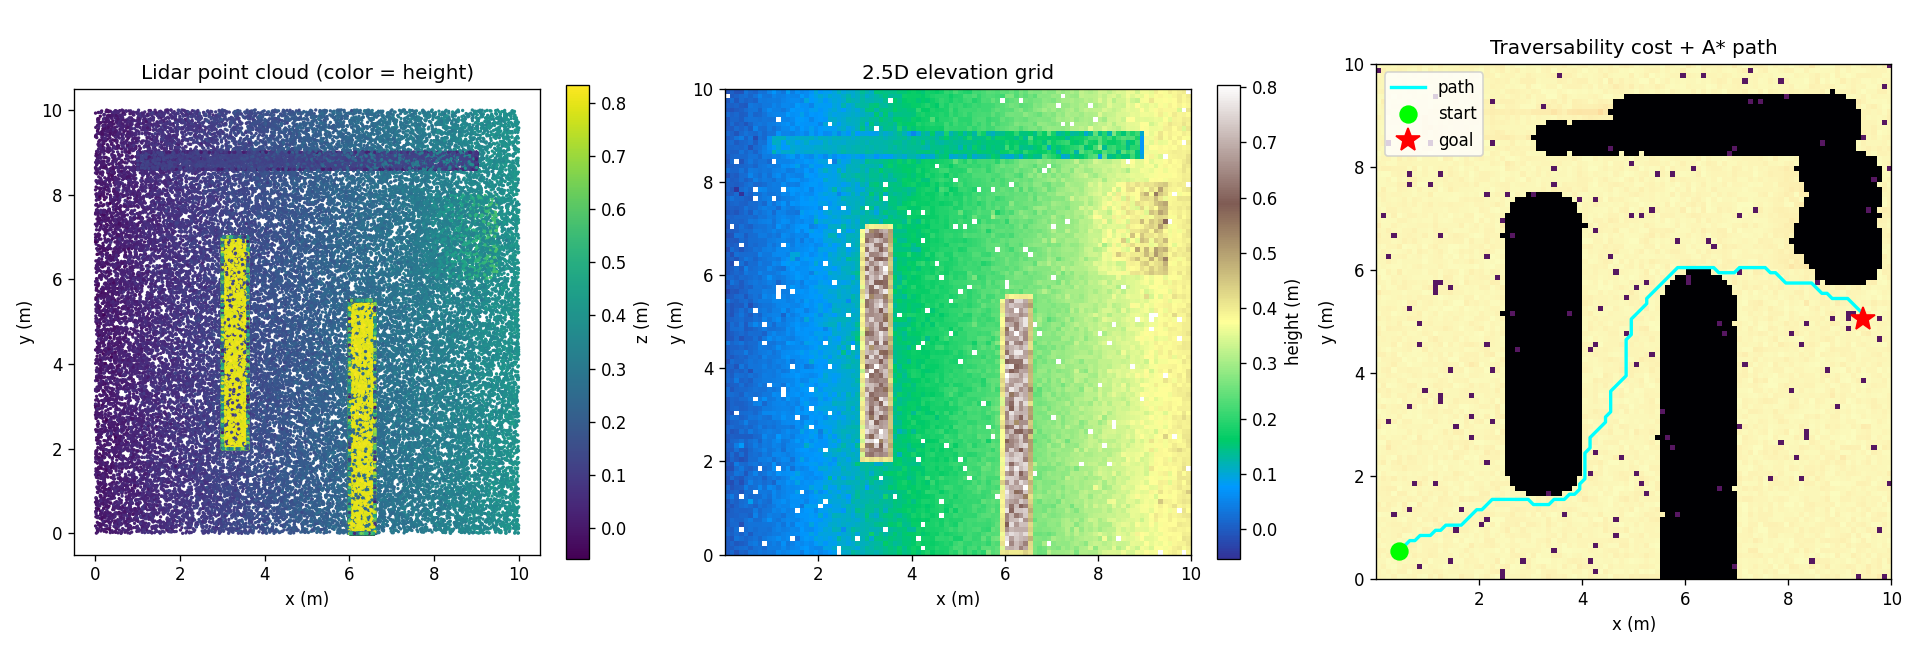
\includegraphics[width=\linewidth]{out.png}
\caption{Synthetic scene. Left: raw point cloud coloured by height. Centre: 2.5D
elevation grid. Right: traversability cost grid with the A$^\star$ path routing
between the two walls.}
\label{fig:synth}
\end{figure}

\subsection{Real automotive LiDAR (KITTI)}
On a Velodyne HDL-64 scan from KITTI \cite{geiger2013}
(Fig.~\ref{fig:kitti}, ${\sim}120$k points), the pipeline produces a sensible road
path \emph{using default parameters}: the sensor sits ${\sim}\SI{1.7}{m}$ above the
ground, coverage is sparse at range (most far cells are \textsc{unknown}), and
obstacles such as vehicles and walls are correctly marked lethal
(Table~\ref{tab:scans}). Clean LiDAR requires no tuning.

\begin{figure}[t]
\centering
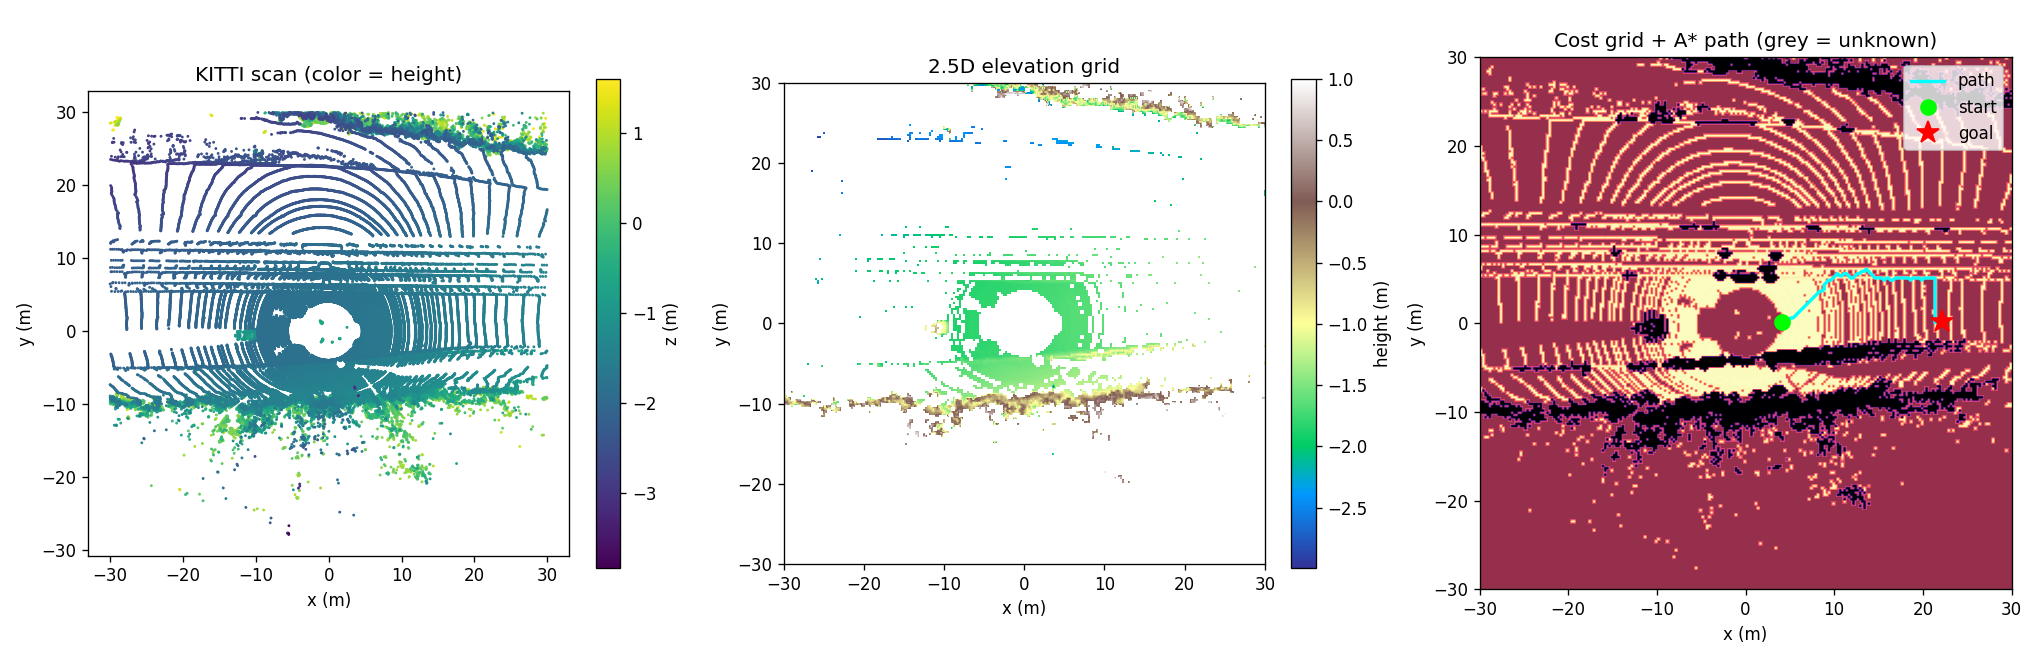
\includegraphics[width=\linewidth]{out_scan1.png}
\caption{Real KITTI scan (\texttt{000001.bin}). Left: scan coloured by height
(Velodyne rings visible). Centre: elevation grid. Right: cost grid with the
planned path; grey is unobserved space.}
\label{fig:kitti}
\end{figure}

\subsection{Real indoor RGB-D and sensor-specific tuning}
On an Open3D indoor room fragment \cite{zhou2018} (Fig.~\ref{fig:room}), the
vertical axis is not gravity-aligned; we auto-detect it from the dominant
height-histogram peak (the floor) and reorient. Critically, a single-view RGB-D
floor exhibits ${\sim}\SIrange{0.15}{0.2}{m}$ of depth scatter \emph{per cell} at
grazing angles, so the default LiDAR thresholds (correctly but unhelpfully) flag
the floor as low-confidence. Loosening $\sigma_{\max}$ and $\theta_{\max}$ and
increasing surface smoothing recovers a traversable floor
(\SI{1.30}{\meter\squared}, Table~\ref{tab:scans}) while keeping $\sim$\SI{80}{\percent} of
furniture cells lethal. \textbf{Lesson:} traversability thresholds encode sensor
\emph{and} robot tolerance and must be matched to the sensor's noise.

\begin{figure}[t]
\centering
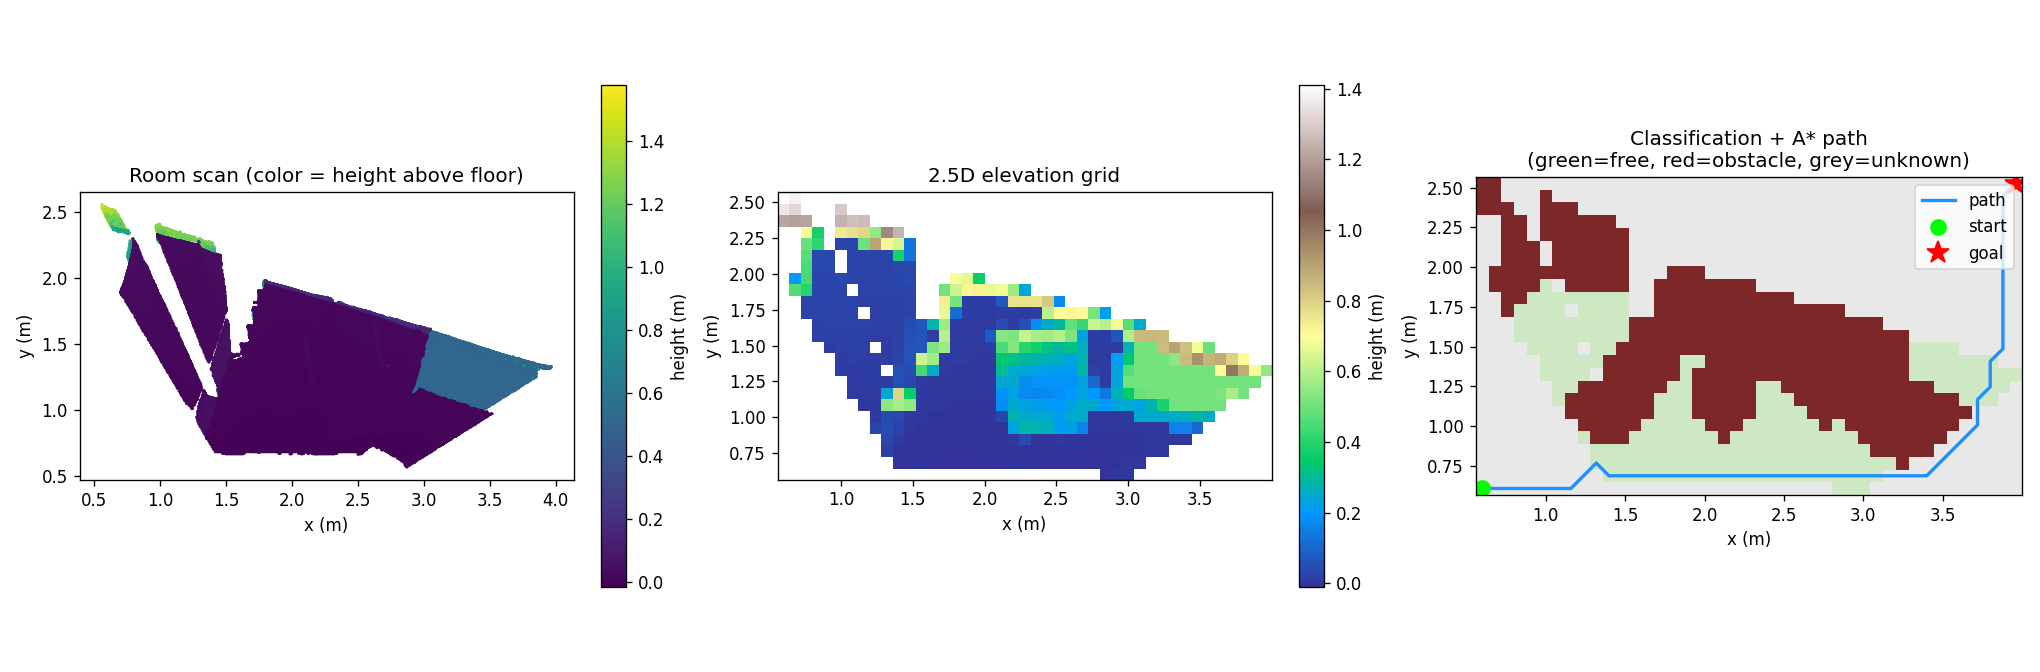
\includegraphics[width=\linewidth]{out_room.png}
\caption{Indoor RGB-D room scan. Left: scan coloured by height above floor.
Centre: elevation grid. Right: classification (green free, red obstacle, grey
unknown) with the path routing around furniture.}
\label{fig:room}
\end{figure}

\begin{table}[t]
\centering
\caption{Per-scan discretization and planning results.}
\label{tab:scans}
\sisetup{group-separator={,}}
\begin{tabular}{lrrrrr}
\toprule
Scene & Points & Obs.\ cells & Lethal & Unknown & Path \\
\midrule
Synthetic        & 85\,002  & 9\,837  & 2\,749 & 163    & \SI{13.3}{m} \\
KITTI 000001     & 120\,268 & 14\,027 & 5\,233 & 43\,573 & \SI{27.6}{m} \\
KITTI 000002     & 126\,891 & 4\,429  & 2\,263 & 53\,171 & \SI{26.3}{m} \\
RGB-D room       & 196\,133 & 528     & 325    & 547    & \SI{4.97}{m} \\
\bottomrule
\end{tabular}
\end{table}

\subsection{Kalman fusion and the need for registration}
Figure~\ref{fig:paper} (left) shows the mean per-cell variance falling
monotonically as scans are fused---the noise reduction the reference method
attributes to Kalman filtering \cite{refpaper,fankhauser2018}. To test
\emph{multi-scan} fusion on real data we fused the two provided KITTI scans.
Table~\ref{tab:fusion} reports a control: fusing a scan with itself (perfectly
aligned) leaves the lethal-cell count unchanged and merely lowers variance,
whereas fusing two consecutive scans inflates lethal cells by
\SI{80}{\percent}. The cause is a pose difference (near-sensor ground at
\SI{-1.67}{m} vs.\ \SI{-0.88}{m}): without scan registration via ICP
\cite{besl1992}, fusing differently-posed scans produces ghosting. \textbf{This is
an empirical demonstration of why the reference stack includes a localization
stage}---our map assumes known poses, which the SLAM/ICP block must supply.

\begin{table}[t]
\centering
\caption{Kalman fusion control on real KITTI scans (\SI{0.25}{m} grid).}
\label{tab:fusion}
\begin{tabular}{lrr}
\toprule
Fusion & Lethal cells & Observed cells \\
\midrule
Scan 1 alone                 & 4\,108 & 14\,027 \\
Scan 1 + Scan 1 (aligned)    & 4\,108 & 14\,027 \\
Scan 1 + Scan 2 (diff.\ pose)& 7\,380 & 15\,910 \\
\bottomrule
\end{tabular}
\end{table}

\subsection{Full stack and person-following}
Figure~\ref{fig:paper} shows the complete fixed-goal stack: Kalman map, Dijkstra
global path (orange), elastic-band smoothing (navy), and APF tracking (blue).
Pure APF toward the far goal stalled \SI{4.4}{m} short in a local minimum at the
walls; the carrot-following two-level scheme reaches the goal within the
\SI{0.15}{m} tolerance while maintaining \SI{0.57}{m} obstacle clearance.
Figure~\ref{fig:follow} shows the person-following mode: a person walks a
guaranteed-free route and the robot APF-tracks them at a mean gap of \SI{0.58}{m}
while avoiding hazards \cite{islam2019}.

\begin{figure}[t]
\centering
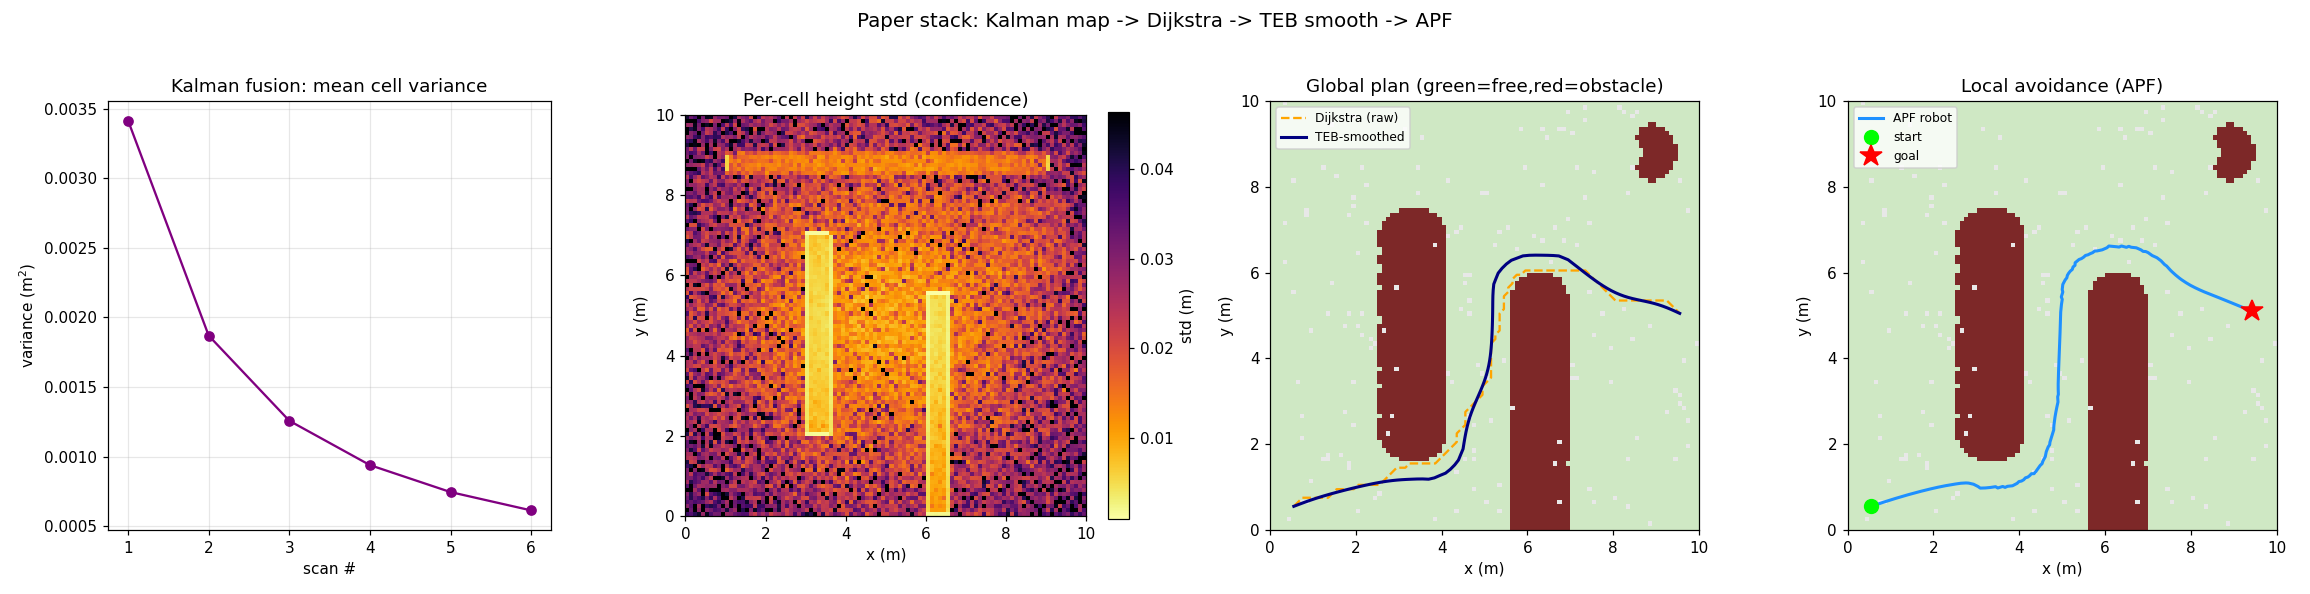
\includegraphics[width=\linewidth]{out_paper.png}
\caption{Paper stack on synthetic terrain. Left: Kalman variance decreasing over
fused scans. Centre-left: per-cell height standard deviation (confidence).
Centre-right: Dijkstra path (orange) and elastic-band-smoothed path (navy).
Right: APF trajectory tracking the smoothed global path.}
\label{fig:paper}
\end{figure}

\begin{figure}[t]
\centering
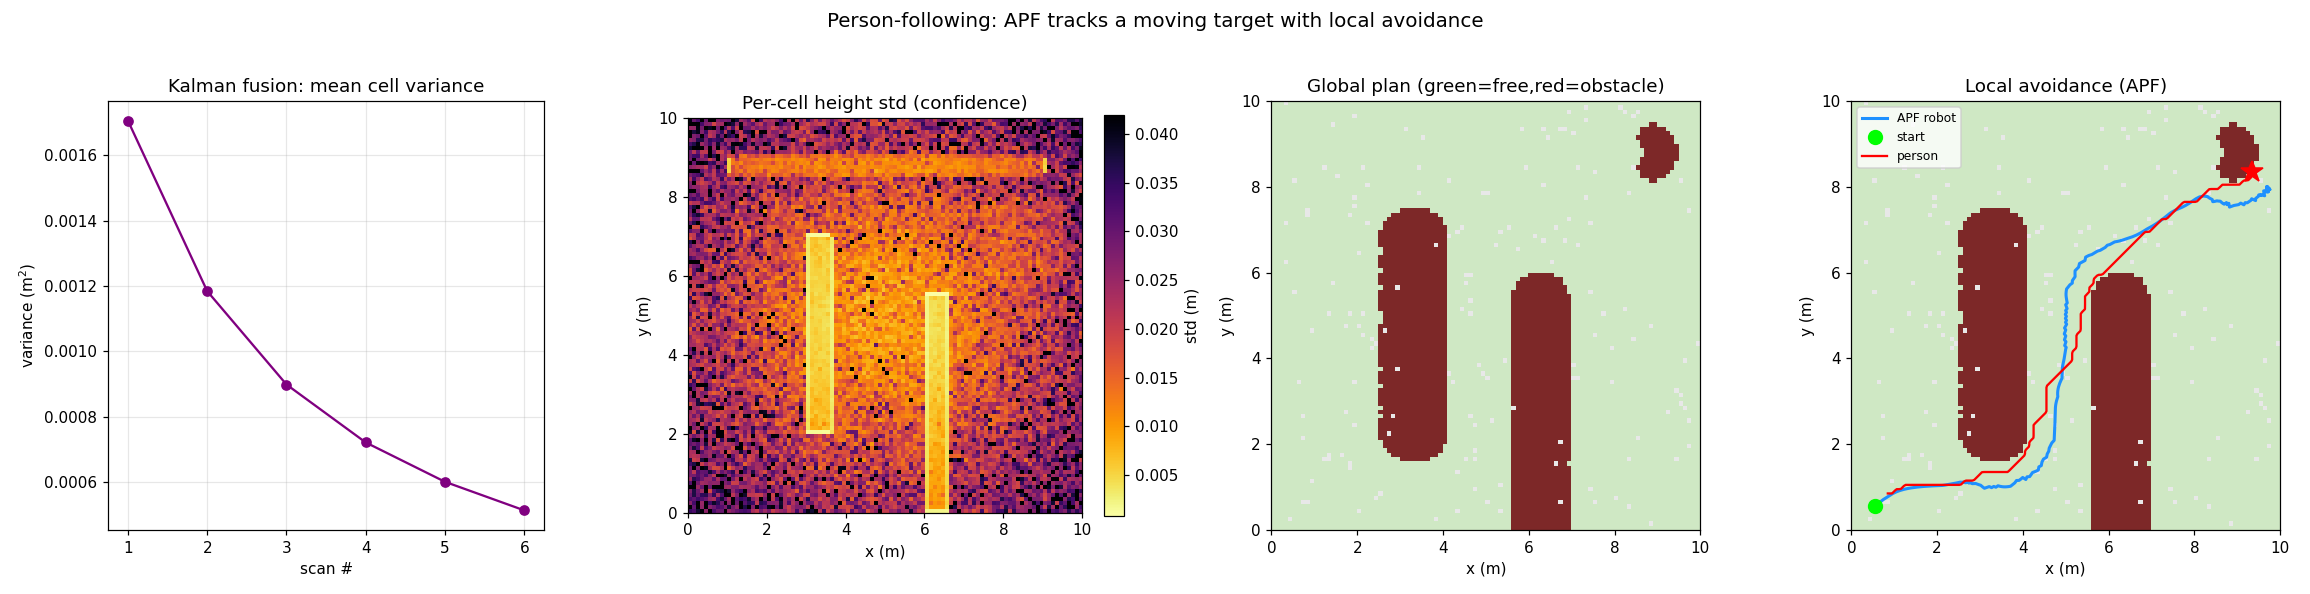
\includegraphics[width=\linewidth]{out_paper_follow.png}
\caption{Person-following. The robot (blue) tracks a moving person (red) with APF
local avoidance around the two walls, at a mean separation of \SI{0.58}{m}.}
\label{fig:follow}
\end{figure}

\subsection{Three-dimensional visualization}
To aid interpretation, the elevation grid is rendered as a 3D surface coloured by
traversability with the path draped on top (Fig.~\ref{fig:viz3d}); an interactive
WebGL version is also produced. The relief makes the relationship between the
route and the standing obstacles immediately legible.

\begin{figure}[t]
\centering
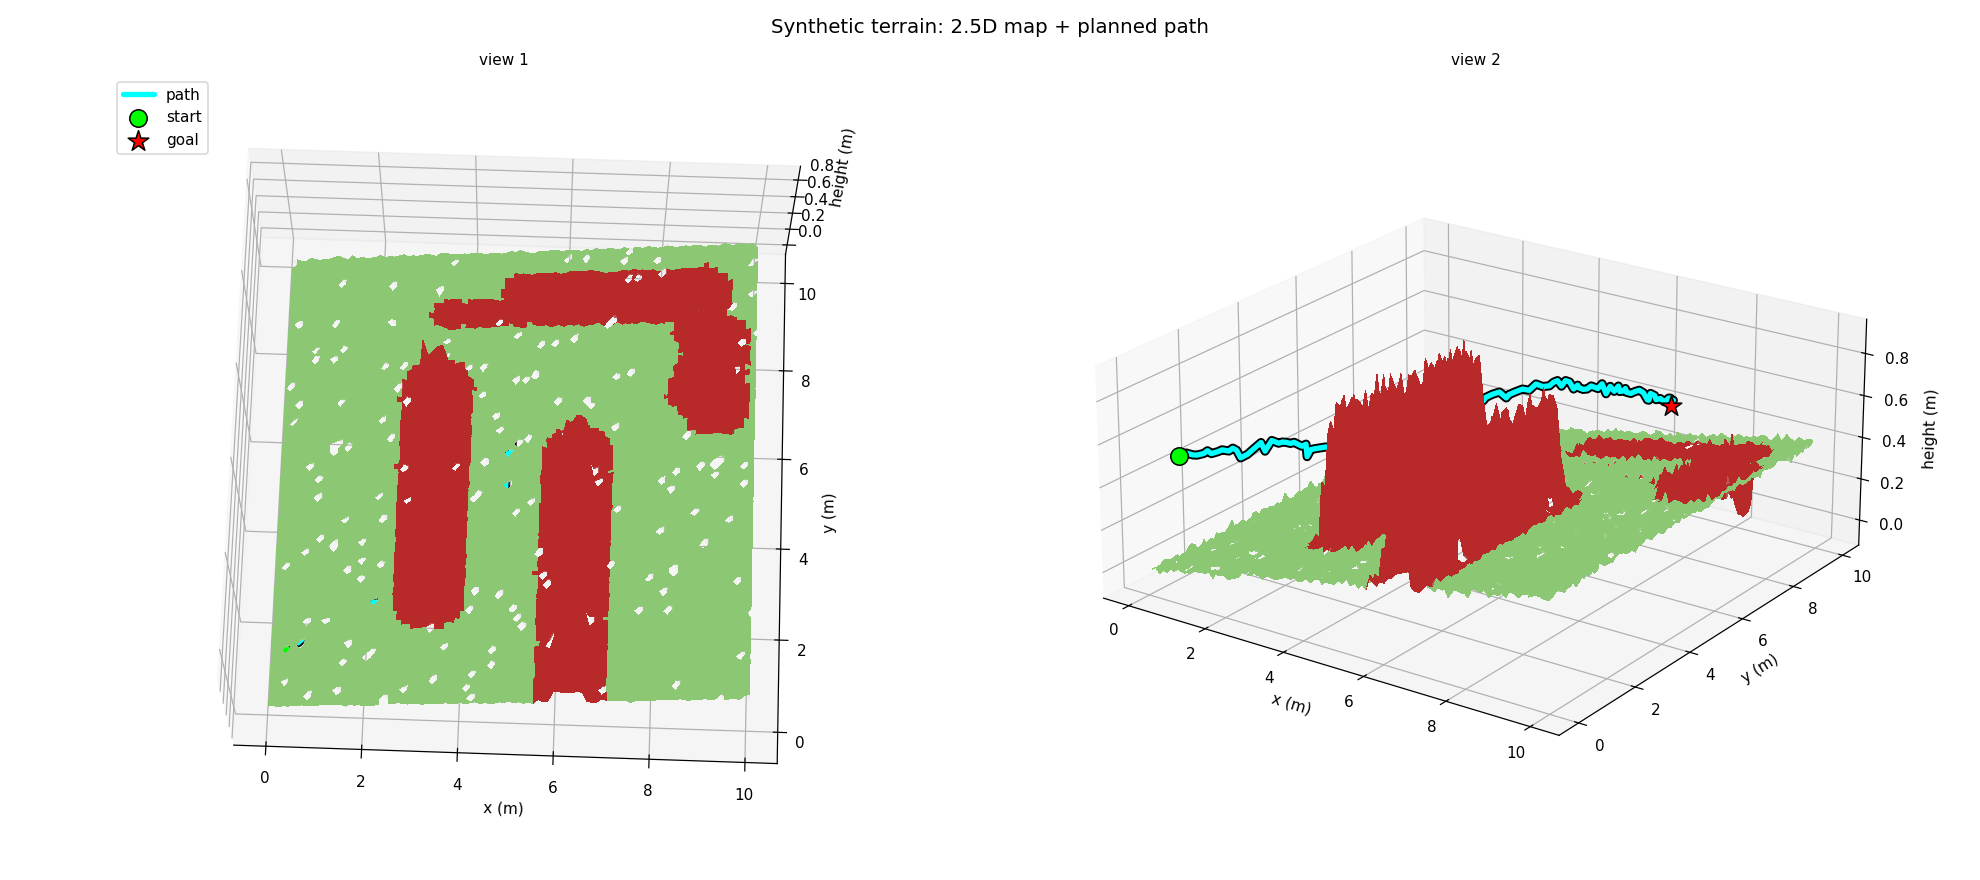
\includegraphics[width=\linewidth]{out_3d.png}
\caption{3D view of the synthetic 2.5D map (two angles). Green is traversable, red
is obstacles (height exaggerated $4\times$); the cyan tube is the planned path
from the green start to the red goal.}
\label{fig:viz3d}
\end{figure}

% ================================================================
\section{Discussion}
\label{sec:discussion}
The experiments yield three transferable findings. First, the same code base
handles clean automotive LiDAR at default settings but requires looser tolerances
and stronger smoothing for noisy single-view RGB-D; traversability thresholds are
not universal constants but sensor-conditioned. Second, the fusion control
(Table~\ref{tab:fusion}) makes concrete why globally-consistent localization is a
prerequisite for multi-scan mapping: without ICP registration \cite{besl1992},
fusion degrades rather than improves the map. Third, the APF local-minimum result
validates the two-level design of the reference stack \cite{refpaper}---a global
planner is not optional decoration but the mechanism that frees the local planner
from terrain traps.

% ================================================================
\section{Limitations and Future Work}
\label{sec:limits}
The principal omission is the SLAM/ICP \emph{localization} block: poses are assumed
known and passed to the map. Closing this loop with a point-to-plane ICP
\cite{besl1992} or an off-the-shelf LiDAR-inertial odometry front-end would enable
true multi-scan fusion on moving-robot data. The smoother is the geometric core of
TEB, not the full time-optimal optimizer \cite{rosmann2017}. For person-following,
a perception front-end (RGB person detection, tracking, and target-position
estimation \cite{islam2019}) is required to supply $q_g(t)$. Finally, on-robot
validation through the Nav2 integration \cite{macenski2020} remains to be done.

% ================================================================
\section{Conclusion}
\label{sec:conclusion}
We reproduced and extended a classical mapping--localization--planning stack for
quadruped navigation \cite{refpaper}, implementing a Kalman-filtered 2.5D terrain
map, Dijkstra/A$^\star$ global planning, elastic-band smoothing, and a Khatib APF
local planner with a person-following mode, plus a Nav2 deployment path. Validation
on synthetic, automotive-LiDAR, and indoor-RGB-D data confirmed the stack functions
on real input and surfaced practical lessons on sensor-specific tuning, the
necessity of scan registration, and the global/local planner division of labour.

\section*{Reproducibility}
The implementation is plain Python (\texttt{numpy}/\texttt{matplotlib}). Figures in
this report are produced directly by the project's demo and example scripts; all
quantitative results are emitted by those scripts and covered by the unit-test
suite.

\bibliographystyle{ieeetr}
\bibliography{references}

\end{document}
